\subsection{Упражнение 1}

«A Soft Murmur» — это веб-сайт, на котором можно послушать множество естественных источников шума, включая дождь, волны, ветер и т. д. 

\noindent На http://asoftmurmur.com/about/ вы можете найти их список записей, большинство из которых находится на http://freesound.org.

\noindent Загрузите несколько таких файлов и вычислите спектр каждого сигнала. Спектр мощности похож на белый шум, розовый шум, или броуновский шум? Как изменяется спектр во времени?

Можно вырезать небольшой отрывок.

\begin{lstlisting}[language=Python]
wave = read_wave('22604__martypinso__dmp010037-crickets-texas.wav')
segment = wave.segment(start=10, duration=1.0)
segment.plot()
\end{lstlisting}
\begin{figure}[H]
	\begin{center}
		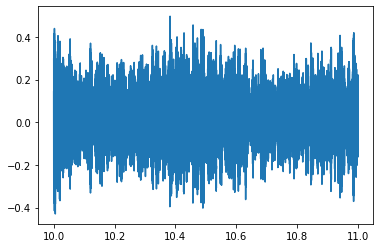
\includegraphics[scale=1]{fig/lab04/lab04_7_0.png}
		\caption{График сигнала}
	\end{center}
\end{figure}

Для определения характеристик шума используем код из пособия по построению графика спекта в логорифмическом масштабе.

\begin{lstlisting}[language=Python]
from thinkdsp import decorate
spectrum.plot_power()

loglog = dict(xscale='log', yscale='log')
decorate(xlabel='Frequency (Hz)',
         ylabel='Power', 
         **loglog)
\end{lstlisting}
\begin{figure}[H]
	\begin{center}
		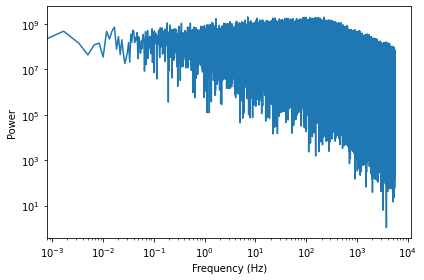
\includegraphics[scale=1]{fig/lab04/lab04_9_0.png}
		\caption{Спектр в логорифмическом масштабе}
	\end{center}
\end{figure}

Давайте возьмём следующий сегмент для наглядности.

\begin{lstlisting}[language=Python]
segment1 = wave.segment(start=11, duration=1.0)
spectrum1 = segment1.make_spectrum()
spectrum.plot_power()
spectrum1.plot_power()


loglog = dict(xscale='log', yscale='log')
decorate(xlabel='Frequency (Hz)',
         ylabel='Power', 
         **loglog)
\end{lstlisting}
\begin{figure}[H]
	\begin{center}
		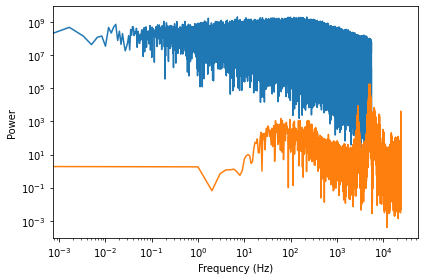
\includegraphics[scale=1]{fig/lab04/lab04_12_0.png}
		\caption{Сравнение спектров в логорифмическом масштабе}
	\end{center}
\end{figure}

\begin{lstlisting}[language=Python]
noise = UncorrelatedGaussianNoise()
wave2 = noise.make_wave(duration=1)
spectrum2 = wave2.make_spectrum()
spectrum.plot_power()
spectrum2.plot_power()


loglog = dict(xscale='log', yscale='log')
decorate(xlabel='Frequency (Hz)',
         ylabel='Power', 
         **loglog)
\end{lstlisting}

Оранжевым обозначен Гауссов шум.

\begin{figure}[H]
	\begin{center}
		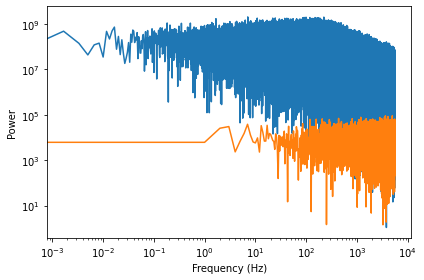
\includegraphics[scale=1]{fig/lab04/lab04_14_0.png}
		\caption{Сравнение нашего звука с Гауссовым шумом}
	\end{center}
\end{figure}

\subsection{Упражнение 2}

Реализуйте метод Бартлетта\cite{barlett} и используйте его для оценки спектра мощности шумового сигнала. Подсказка: посмотрите на реализацую make\_spectrogram.

Исходя из статьи на википедии надо поделить данные на сегменты, потом для каждого сегмента сделать разложение Фурье, вычислить сумму квадратов и раздлелить на количество элементов и взять от этого всего корень.

Посмотрим с помощью чего и как создаются спектограммы:

\begin{lstlisting}[language=Python]
    def make_spectrogram(self, seg_length, win_flag=True):
        """Computes the spectrogram of the wave.
        seg_length: number of samples in each segment
        win_flag: boolean, whether to apply hamming window to each segment
        returns: Spectrogram
        """
        if win_flag:
            window = np.hamming(seg_length)
        i, j = 0, seg_length
        step = int(seg_length // 2)

        # map from time to Spectrum
        spec_map = {}

        while j < len(self.ys):
            segment = self.slice(i, j)
            if win_flag:
                segment.window(window)

            # the nominal time for this segment is the midpoint
            t = (segment.start + segment.end) / 2
            spec_map[t] = segment.make_spectrum()

            i += step
            j += step

        return Spectrogram(spec_map, seg_length)
\end{lstlisting}
\begin{lstlisting}[language=Python]
        """Initializes a spectrum.
        hs: array of amplitudes (real or complex)
        fs: array of frequencies
        framerate: frames per second
        full: boolean to indicate full or real FFT
        """
        self.hs = np.asanyarray(hs)
        self.fs = np.asanyarray(fs)
        self.framerate = framerate
        self.full = full
\end{lstlisting}

Для создания своей функции надо изменять словарь:
\begin{lstlisting}[language=Python]
def make_barlett(wave, N, flag=True):
  spectrogram = wave.make_spectrogram(N,flag)
  spec_mac = spectrogram.spec_map.values()

  powers = []
  for spectrum in spec_mac:
    powers.append(spectrum.power)
  
  hs = np.sqrt(sum(powers)/ len(powers))
  fs = next(iter(spec_mac)).fs

  return Spectrum(hs, fs, wave.framerate)
\end{lstlisting}

\begin{lstlisting}[language=Python]
barlett = make_barlett(segment,1024)
barlett.plot_power()

decorate(xlabel='Frequency (Hz)', 
         ylabel='Power', 
         **loglog)
\end{lstlisting}
\begin{figure}[H]
	\begin{center}
		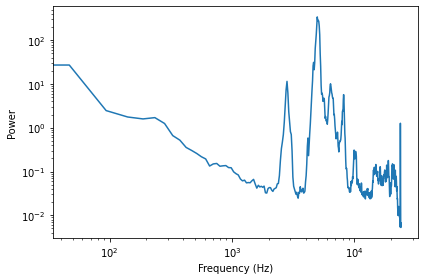
\includegraphics[scale=1]{fig/lab04/lab04_23_0.png}
		\caption{Результат}
	\end{center}
\end{figure}


\subsection{Упражнение 3}

Загрузите в виде CSV-файла исторические данные о ежедневной цене BitCoin. Откройте этот файл и вычислите спектр цен BitCoin как функцию времени. Похоже ли это на белый, розовый или броуновский шум?

\begin{lstlisting}[language=Python]
  if not os.path.exists('market-price.csv'):
    !wget https://github.com/wooftown/spbstu-telecom/raw/main/Content/market-price.csv
\end{lstlisting}
\begin{lstlisting}[language=Python]
import csv

worth = []

with open('market-price.csv') as File:
  reader = csv.reader(File, delimiter=',', quotechar=',',
                        quoting=csv.QUOTE_MINIMAL)
  worth = [row[1] for row in reader]

worth = worth [1:]
days = a=np.arange(0,len(worth))
\end{lstlisting}
\begin{lstlisting}[language=Python]
wave = Wave(worth,days,1)
wave.plot()
decorate(xlabel='Time (days)')
\end{lstlisting}
\begin{figure}[H]
	\begin{center}
		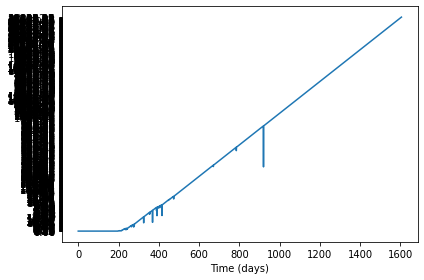
\includegraphics[scale=1]{fig/lab04/lab04_28_0.png}
		\caption{График цен BitCoin}
	\end{center}
\end{figure}

График получился не очень красивым из-за того, что слишком много данных, можно приблизить и посмотреть какой-то один сегмент. Давайте перейдём к спектограмме.

\begin{lstlisting}[language=Python]
spectrum = wave.make_spectrum()
spectrum.plot_power()
decorate(xlabel='Frequency (1/days)',
         ylabel='Power', 
         **loglog)
\end{lstlisting}
\begin{figure}[H]
	\begin{center}
		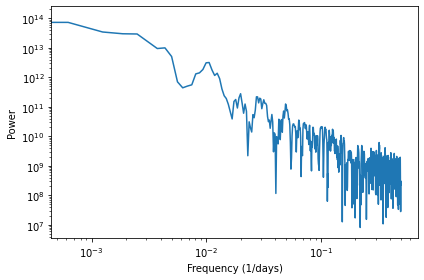
\includegraphics[scale=1]{fig/lab04/lab04_32_0.png}
		\caption{Спектрограмма цен BitCoin в логорифмическом формате}
	\end{center}
\end{figure}

Больше всего это походе на красный шум, так как связь похожа на отбраную квадратную.

\subsection{Упражнение 4}

Счетчик Гейгера — это прибор, который регистрирует радиацию. Когда ионизирующая частица попадает на детектор, он генерирует всплеск тока. Общий вывод в определенный момент времени можно смоделировать как некоррелированный шум Пуассона (UP), где каждая выборка представляет собой случайную величину из распределения Пуассона, которая соответствует количеству частиц, обнаруженных в течение интервала.

Напишите класс с именем `UncorrelatedPoissonNoise`, который наследуется от `\_Noise` и предоставляет `evaluate`. Он должен использовать `np.random.poisson` для генерации случайных значений из распределения Пуассона. Параметр этой функции, lam, представляет собой среднее число частиц в течение каждого интервала. Вы можете использовать атрибут `amp`, чтобы указать `lam`. Например, если частота кадров равна 10 кГц, а amp равно 0,001, мы ожидаем около 10 «кликов» в секунду.

Создайте около секунды шума UP и послушайте его. Для низких значений «ампер», например 0,001, это должно звучать как счетчик Гейгера. Для более высоких значений это должно звучать как белый шум. Вычислите и начертите спектр мощности, чтобы увидеть, похож ли он на белый шум.

\begin{lstlisting}[language=Python]
class UncorrelatedPoissonNoise(Noise):
  def evaluate(self, ts):
    ys = np.random.poisson(self.amp,len(ts))
    return ys
\end{lstlisting}
\begin{lstlisting}[language=Python]
noise1 = UncorrelatedPoissonNoise(0.001)
wave1 = noise1.make_wave(duration=1,framerate = 11025)
wave1.plot()
\end{lstlisting}
\begin{figure}[H]
	\begin{center}
		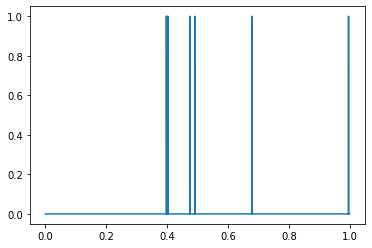
\includegraphics[scale=1]{fig/lab04/lab04_37_0.png}
		\caption{Получившийся сигнал}
	\end{center}
\end{figure}

\begin{lstlisting}[language=Python]
noise2 = UncorrelatedPoissonNoise(1)
wave2 = noise2.make_wave(duration=1,framerate = 11025)
wave2.plot()
\end{lstlisting}
\begin{figure}[H]
	\begin{center}
		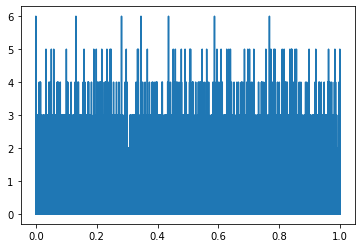
\includegraphics[scale=1]{fig/lab04/lab04_39_0.png}
		\caption{Получившийся сигнал}
	\end{center}
\end{figure}
\begin{lstlisting}[language=Python]
spectrum1 = wave1.make_spectrum()
spectrum2 = wave2.make_spectrum()
spectrum1.plot_power()
spectrum2.plot_power()

decorate(xlabel='Frequency (Hz)', 
         ylabel='Power', 
         **loglog)
\end{lstlisting}
\begin{figure}[H]
	\begin{center}
		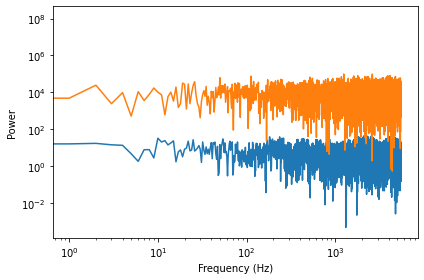
\includegraphics[scale=1]{fig/lab04/lab04_41_0.png}
		\caption{Сравнение спектров}
	\end{center}
\end{figure}

При увеличении значения ампилутуды сигнал всё больше походит на белый шум.
\subsection{Упражнение 5}

В этой главе описан алгоритм генерации розового шума. Концептуально простой, но вычислительно затратный. Есть более эффективные альтернативы, такие как алгоритм Восса-Маккартни.

\noindent Исследуйте этот метод, реализуйте его, вычислите спектр и подтвердите, что он имеет желаемое отношение между мощностью и частотой.

\begin{lstlisting}[language=Python]
def iterpink(depth):
    values = np.random.randn(depth)
    smooth = np.random.randn(depth)
    source = np.random.randn(depth)
    sumvals = values.sum()
    i = 0
    while True:
        yield sumvals + smooth[i]
        i += 1
        if i == depth:
            i = 0
            smooth = np.random.randn(depth)
            source = np.random.randn(depth)
            continue
        c = 0
        while not (i >> c) & 1:
            c += 1
        sumvals += source[i] - values[c]
        values[c] = source[i]
\end{lstlisting}

\begin{lstlisting}[language=Python]
def pink_noise(points, depth=16):
    a = []
    s = iterpink(depth)
    for n in range(points):
        a.append(next(s))
    return np.array(a)
\end{lstlisting}

\begin{lstlisting}[language=Python]
ys = pink_noise(11025,16)
wave = Wave(ys)
wave.plot()
\end{lstlisting}
\begin{figure}[H]
	\begin{center}
		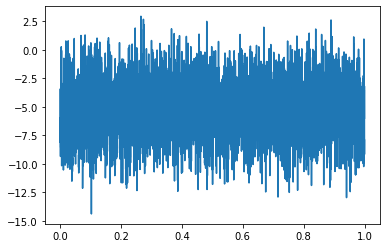
\includegraphics[scale=1]{fig/lab04/lab04_47_0.png}
		\caption{Сгенерированный сигнал}
	\end{center}
\end{figure}

В итоге получили сигнал розового шума:
\begin{lstlisting}[language=Python]
spectrum = wave.make_spectrum()
spectrum.hs[0] = 0
spectrum.plot_power()
decorate(xlabel='Frequency (Hz)',
         ylabel='Power',
         **loglog)
\end{lstlisting}
\begin{figure}[H]
	\begin{center}
		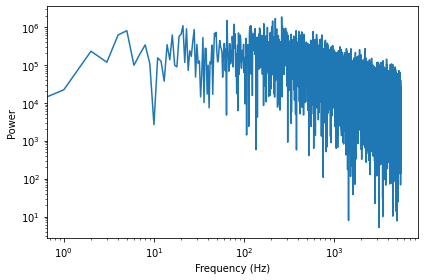
\includegraphics[scale=1]{fig/lab04/lab04_50_0.png}
		\caption{Розовый шум}
	\end{center}
\end{figure}

\subsection{Вывод}

В этой работе был рассмотрен шум. Шум - сигнал, содержащий компоненты с самыми разными частотами, но не имеющий гармонической структуры периодических сигналов, рассмотреных в предыдущих работах.